% Supporting Information for
% "Structure-Aware Row Scaling for Block-Structured Mixed-Integer Programs"
% Build: xelatex supporting-information (or pdflatex; no Wiley class needed)
\documentclass[11pt]{article}
\usepackage[a4paper,margin=2.5cm]{geometry}
\usepackage[T1]{fontenc}
\usepackage{newtxtext,newtxmath}
\usepackage{graphicx}
\usepackage{subcaption}
\usepackage[labelfont=bf]{caption}
\usepackage[colorlinks=true,linkcolor=blue!60!black]{hyperref}

\graphicspath{{figs/}}
\renewcommand{\thefigure}{S\arabic{figure}}

\begin{document}

\begin{center}
{\large\bfseries Supporting Information}\\[0.5em]
\emph{Structure-Aware Row Scaling for Block-Structured Mixed-Integer Programs}\\[0.3em]
Mathias Rodr\'iguez Castro
\end{center}

\bigskip
\noindent This document contains the $0.1\%$-MIPGap Gurobi distributional, diagnostic, and
performance-profile views (Scenario~2 of the main text). They mirror the corresponding
$1\%$-MIPGap figures of the main text; the quantitative evidence for the scenario is in the
main text tables.

\begin{figure}[!htbp]
\centering
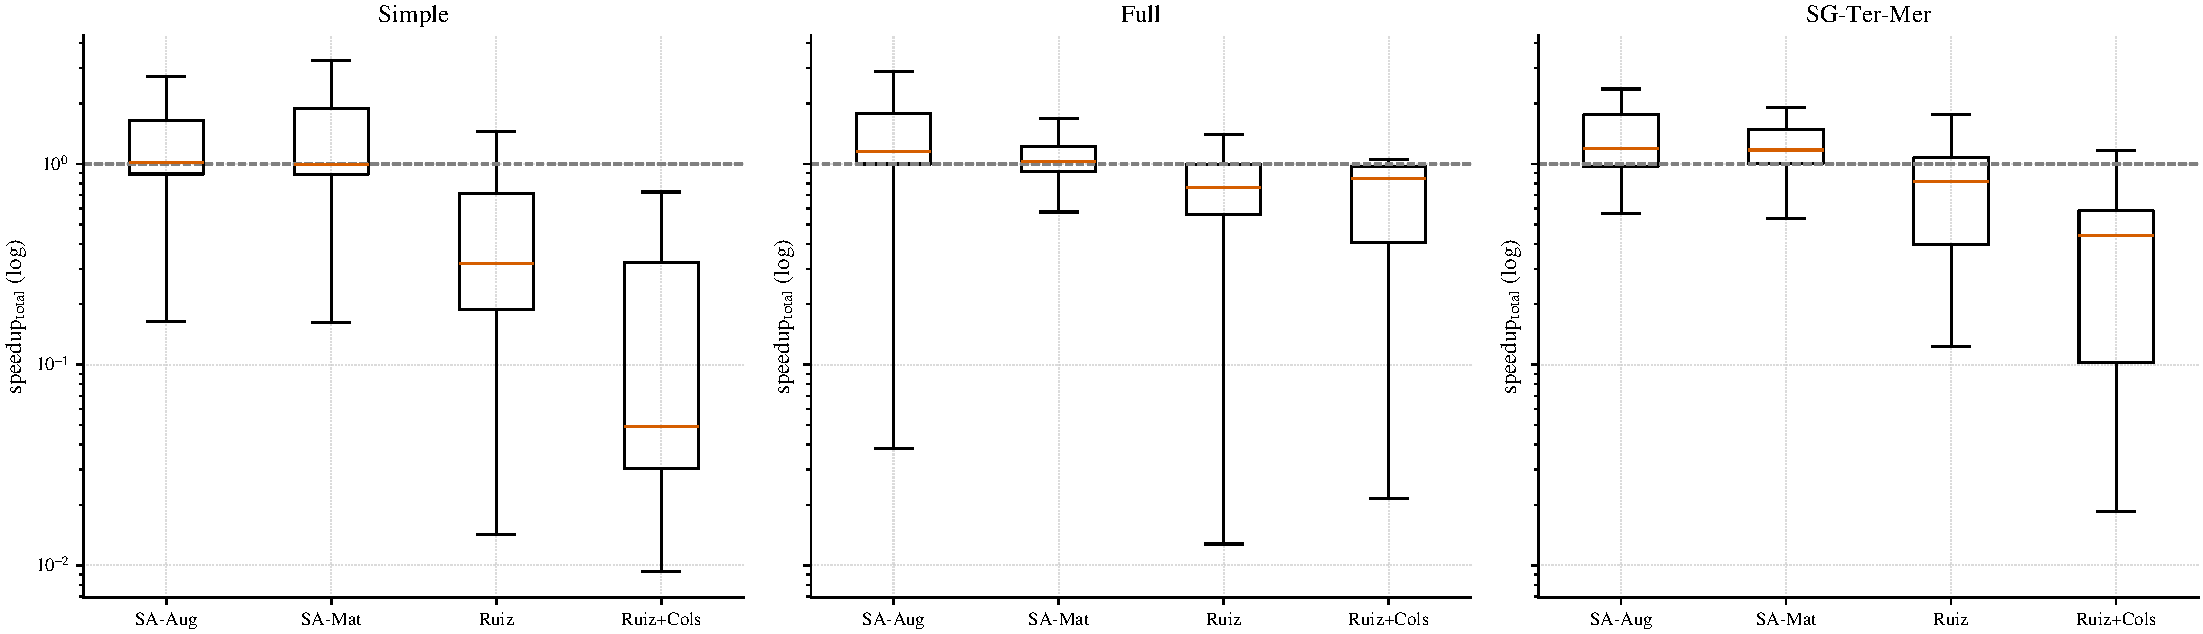
\includegraphics[width=\textwidth]{esc2_gurobi_01pct_boxplot.pdf}
\caption{At $0.1\%$ MIPGap, the Gurobi speedup distributions preserve the same qualitative
pattern observed at the looser tolerance. Values above one indicate faster runs than the
unscaled formulation.}
\label{fig:si-boxplot-gap01}
\end{figure}

\begin{figure}[!htbp]
\centering
\begin{subfigure}[t]{0.485\textwidth}\centering
  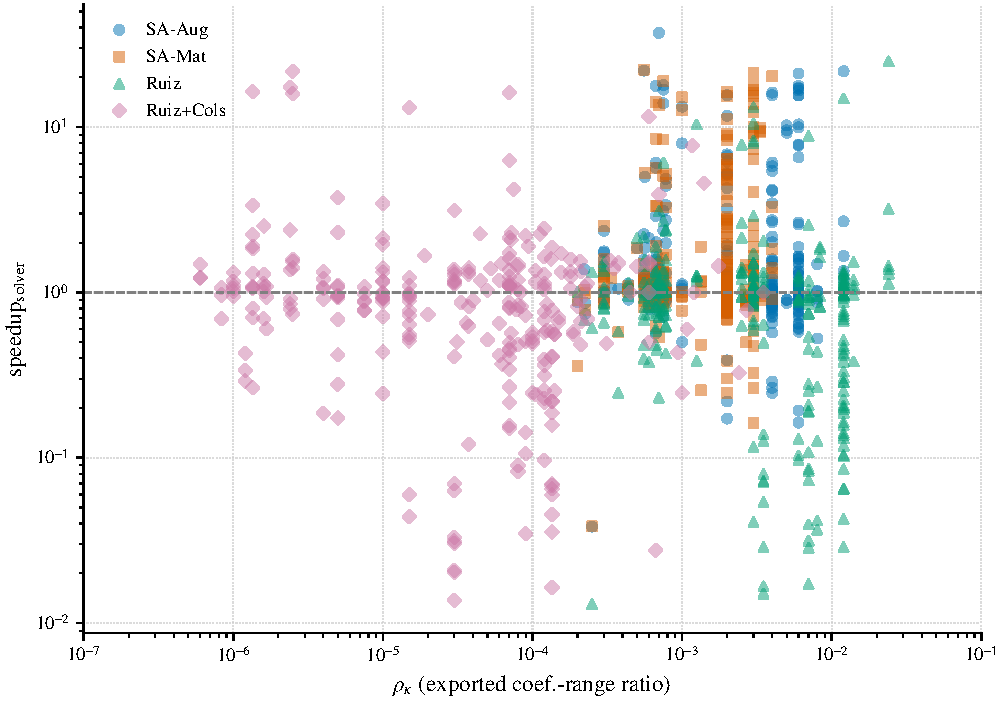
\includegraphics[width=\linewidth]{esc2_gurobi_01pct_scatter_rho.pdf}
  \caption{Static coefficient-range ratio.}
\end{subfigure}\hfill
\begin{subfigure}[t]{0.485\textwidth}\centering
  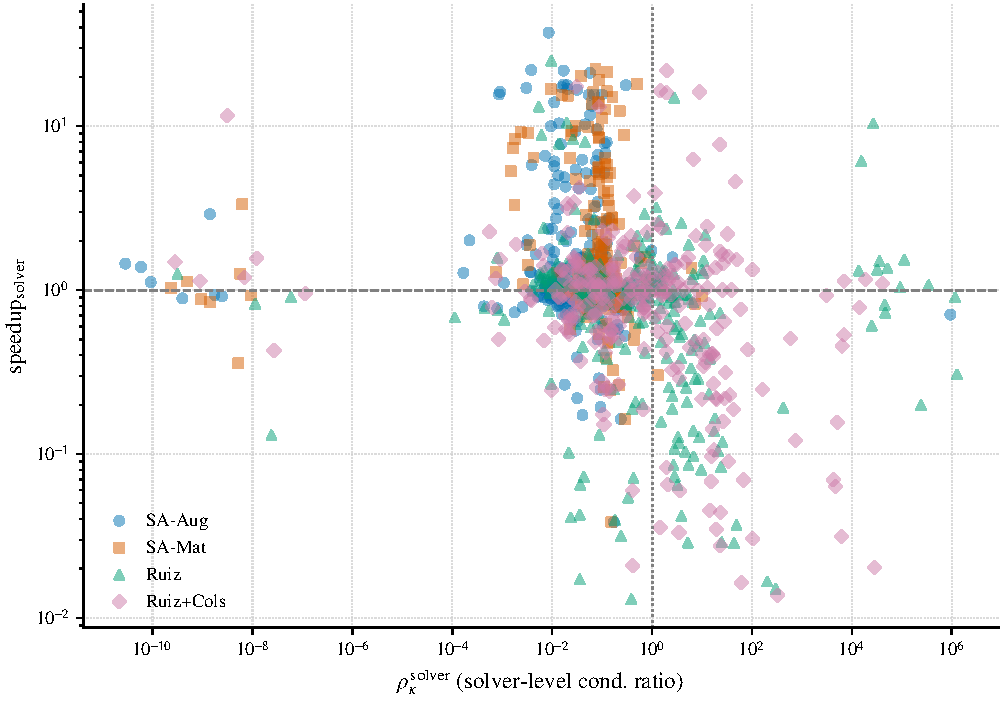
\includegraphics[width=\linewidth]{esc2_gurobi_01pct_scatter_rhosolver.pdf}
  \caption{Solver-level conditioning ratio.}
\end{subfigure}
\caption{At $0.1\%$ MIPGap, the stricter Gurobi runs again separate static coefficient
compression from solver-facing numerical behavior. The solver-level diagnostic remains more
informative than the exported coefficient-range ratio.}
\label{fig:si-scatter-gap01}
\end{figure}

\begin{figure}[!htbp]
\centering
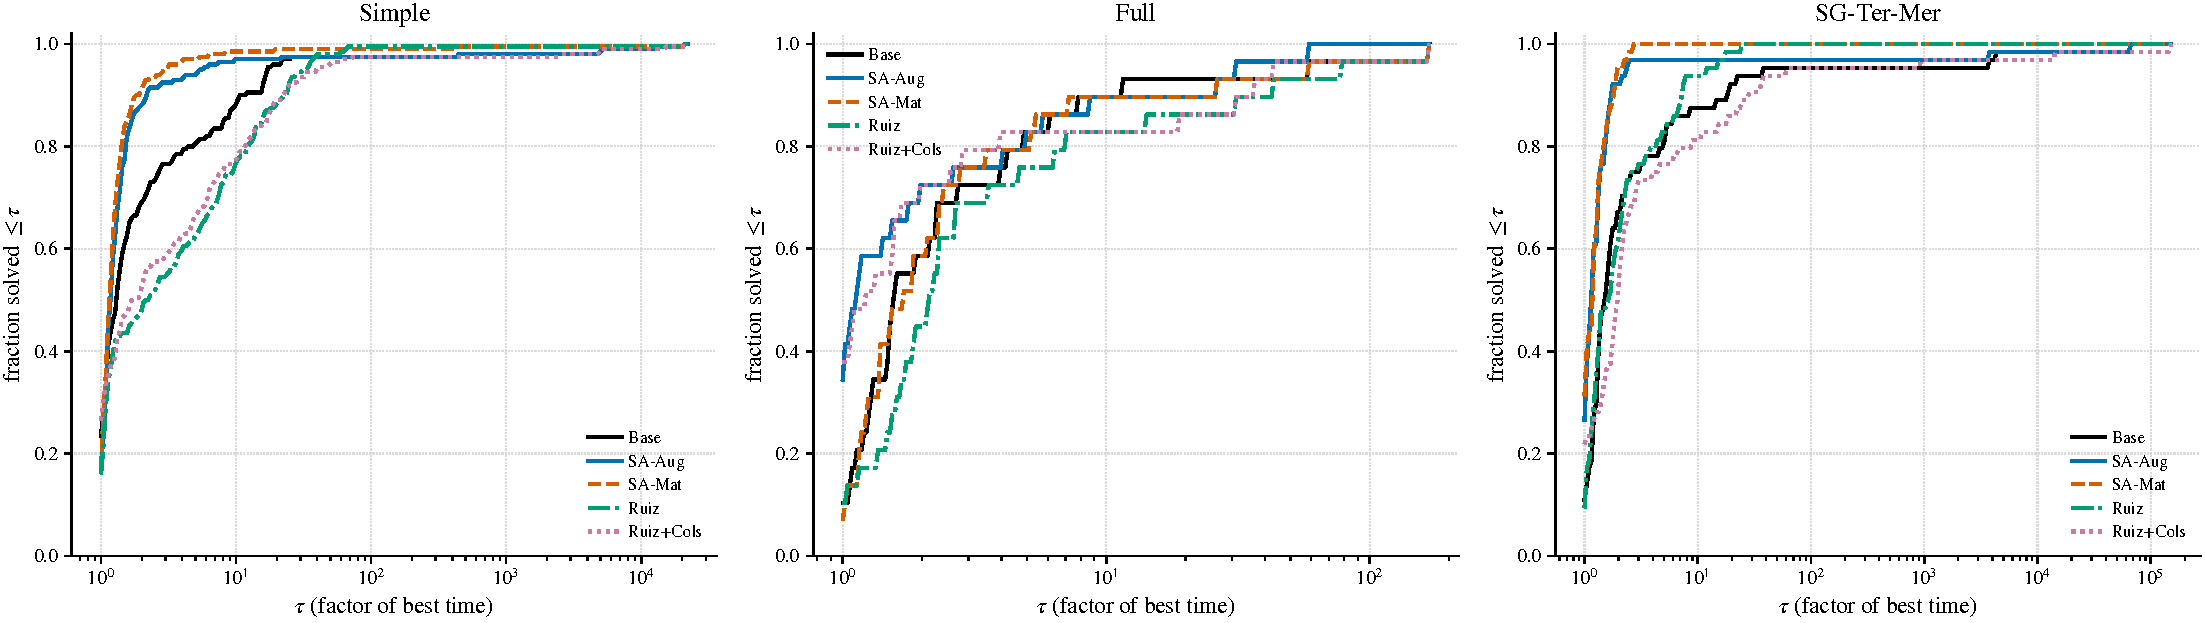
\includegraphics[width=\textwidth]{esc2_gurobi_01pct_perfil.pdf}
\caption{At $0.1\%$ MIPGap, the Dolan--Mor\'e profiles test whether the Gurobi speedups
persist across the heterogeneous instance pool rather than only in averages.}
\label{fig:si-profile-gap01}
\end{figure}

\end{document}
